\chapter{Structural view}

\section{Introduction}
This chapter describes the structural architecture of the system in a top down approach.\\
The blocks are derived from previous documentation.


\section{System overview}
The system consist of a central data unit(CDU) and n number of sensor nodes (SN).\\
Through the 1-wire bus on which all sensor nodes are serially connected both power and communication to all sensors are carried. Below is shown a figure of the system overall blocks and interfaces.
\begin{figure}[hbpt]
\centering
\includegraphics[width=.9\textwidth]{billeder/systembdd}
\caption{System block definition diagram}
\label{systembdd}
\end{figure}

\subsection{General interfaces}
From the CDU power needs to be transmitted to all sensors. As per design, the CDU needs to output 5 volts for every sensor along with 0.7 volts for sensors to be able to respond.\\
Each sensor has a 5V voltage-drop to power the sensor. The response is max 0.7 volts. A formula explains the power needed to power the bus $5V * n + 0.7V$.

\begin{table}[H]
\begin{center}
\begin{tabular}{ p{2.5cm} p{2cm} p{2cm} p{7cm} }
\hline
\textbf{Block} & \textbf{IO} & \textbf{Levels} & \textbf{Description} \\\hline
\multirow{2}{2.5cm}[-3.5em]{CDU} & Sensors\_pos & Min. 10V & The possitive voltage out from the CDU is supplied to the first sensor. The level must be sufficient to supply the number of sensors connected(n).\\ \cline{2-4}
 & Sensors\_neg & NA & The negative port on the CDU is connected to the last sensors in the system and thereby ends the sensor loop. \\ \hline
\multirow{2}{2.5cm}[-3em]{Sensor node} & In\_pos & In\_neg+5V &The In\_pos is where the high potential voltage is supplied to the sensor node. \\ \cline{2-4}
& In\_neg & NA & The negative port at the sensor node is looped to the possitive port on the next sensor or on the "Sensors\_neg" at the CDU. \\ \hline
\end{tabular}
\end{center}
\end{table}

\subsection{Block responsibility}
\subsubsection{CDU}
The CDU contacts each sensor to collect the data values. This is then stored for later extraction.

\subsubsection{Sensor node n}
The sensor node measures temperature.

\section{Detailed block overview}
Below are detailed figures for each block in the system.\\
The blocks in the figures are conceptual blocks and most of them consist of both software and hardware.\\
All the blocks are needed to fulfil the current functionality and requirements of the system. Supporting blocks might be added if the functionality does not fit into the current blocks.

\subsection{CDU}

\begin{figure}[hbpt]
\centering
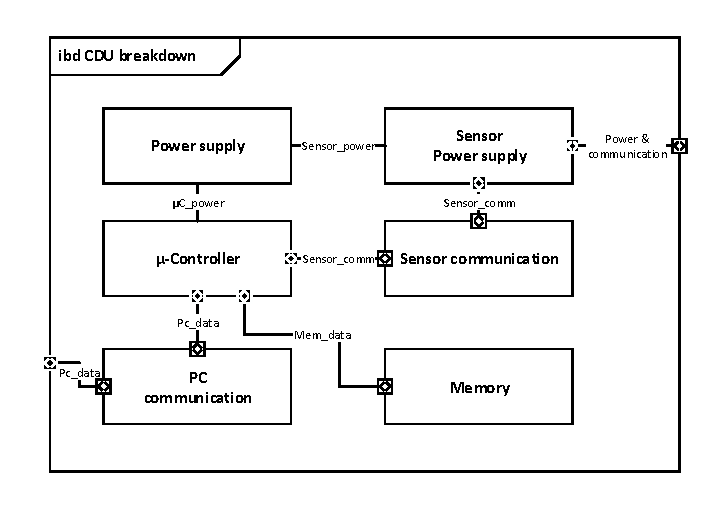
\includegraphics[width=.8\textwidth]{billeder/CDU_IBD}
\caption{Internal Block Diagram of the CDU}
\label{CDU_IBD}
\end{figure}

\subsubsection{Block description}

\textbf{Power supply:}\\
The power supply feeds the necessary power to the modules on which it is connected.\\

\textbf{Sensor power supply:}\\
The Sensor power supply feeds the power needed to operate all sensors connected to the system.\\

\textbf{µ-Controller:}\\
The µ-Controller runs the main application. Main objectives:\\
$\bullet$ Keep track of sensors\\
$\bullet$ Collect data\\
$\bullet$ Store data\\
$\bullet$ Manage communication protocol\\

\textbf{Sensor communication:}\\
The Sensor communication interfaces with the sensor power supply to modulate the power line to the sensor nodes.\\
The sensor communication block has no intelligence and the protocol is handled by the µ-Controller block.\\

\textbf{Memory:}\\
The memory stores all data collected by the µ-Controller. The memory can be detachable or some kind of eeprom/flash.\\

\textbf{PC communication:}\\
The PC communication is an interface to a PC.\\


\subsection{Sensor node n}

\begin{figure}[hbpt]
\centering
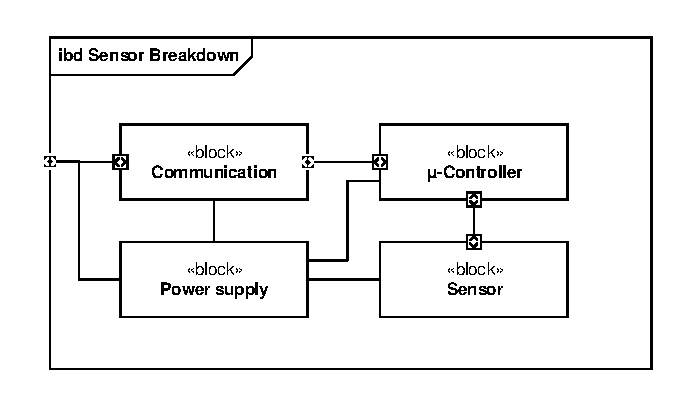
\includegraphics[width=.8\textwidth]{billeder/Sensor_IBD}
\caption{Internal Block Diagram of the sensor}
\label{Sensor_IBD}
\end{figure}

\subsubsection{Block description}

\textbf{Power supply:}\\
The power supply located in the sensor regulates the voltage and current levels to fit the need of the individual blocks in the sensor.\\

\textbf{Communication:}\\
The communication block demodulates the communcation on the input line and feeds it to the sensor logic.\\

\textbf{Logic handler;}\\
The logic handler interprets the incomming communication and responds accordingly.\\
It also handles communication with the Sensor block.\\

\textbf{Sensor:}\\
The sensor block is a complete measurement system with a digital interface.\\



